%%%%%%%%%%%%%%%%%%%%%%%%%%%%%%%%%%%%%%%%%%%%%%%%%%%%%%%%%%%%%%%%%%%%%%%%%%%%%%%%
% template_subtraction.tex: Chapter on Template Subtraction
%%%%%%%%%%%%%%%%%%%%%%%%%%%%%%%%%%%%%%%%%%%%%%%%%%%%%%%%%%%%%%%%%%%%%%%%%%%%%%%%
\chapter{Template Subraction}
\label{template_subtraction_chapter}
%%%%%%%%%%%%%%%%%%%%%%%%%%%%%%%%%%%%%%%%%%%%%%%%%%%%%%%%%%%%%%%%%%%%%%%%%%%%%%%%

%The continuously rotating half-wave plate leaves an optical signal (at [$\1*f_{hwp_rotation}, 2*f_{hwp_rotation}, ..., n*f_{hwp_rotation}$]). 4f and 2f are physically motivated by ... . 1f is there because of rotation. Other harmonics are present because ... . This optical half-wave plate signal is 

The polarized signal we are after resides in the sidebands of 4*f. Put there by the modulation of the gondola scanning sky. 

Our goal is to remove the \ac{HWP} signal from the timestreams such that the residual template is within the detector white noise level in the optical signal band. 

%We model the template as:
%\be
%$\[\beta_t] = \sum_{n=1}^{10}$
%\ee

%\begin{figure}[htbp]
%\begin{center}
%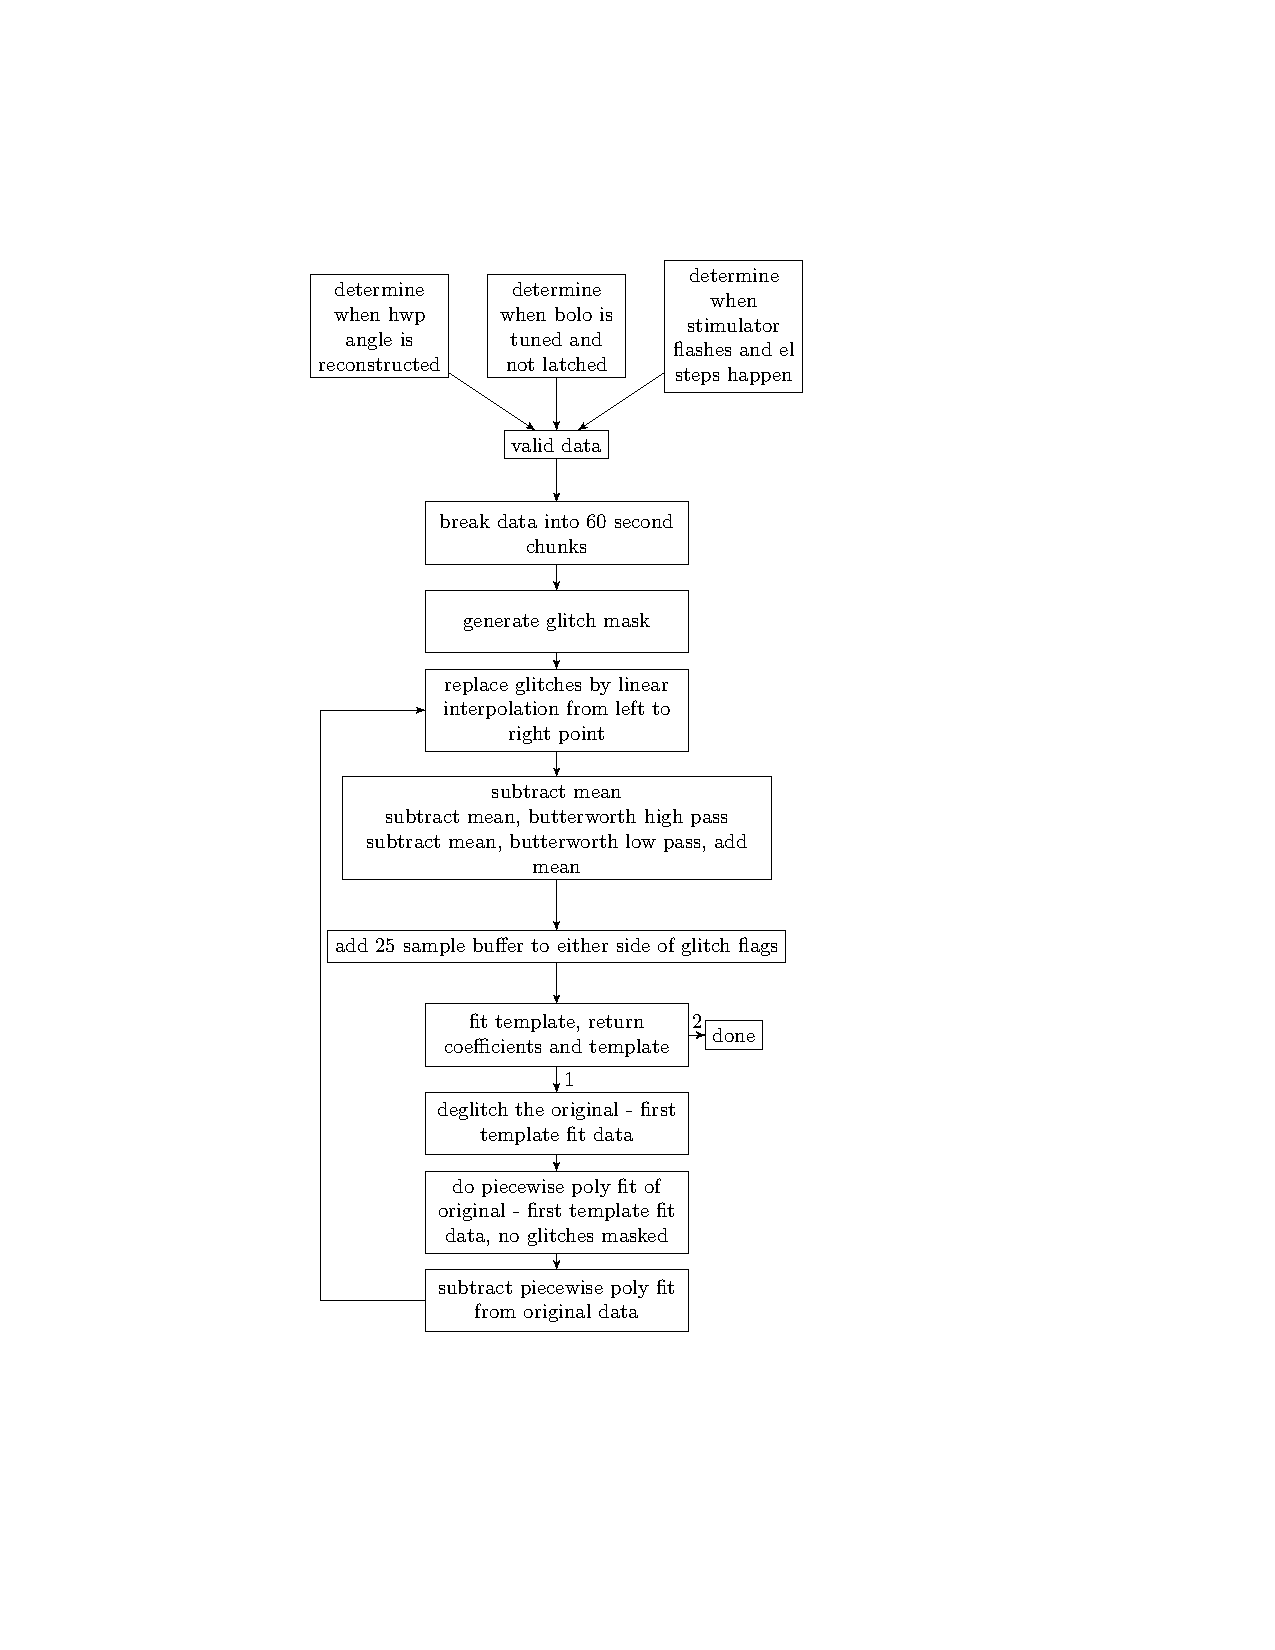
\includegraphics[width=0.6\columnwidth]{figures/template_fit_block_diagram.pdf}
%\caption{Template fit flowchart.}
%\label{fig:template_fit_flow}
%\end{center}
%\end{figure}
%
%
%
%\begin{figure}[htbp]
%\begin{center}
%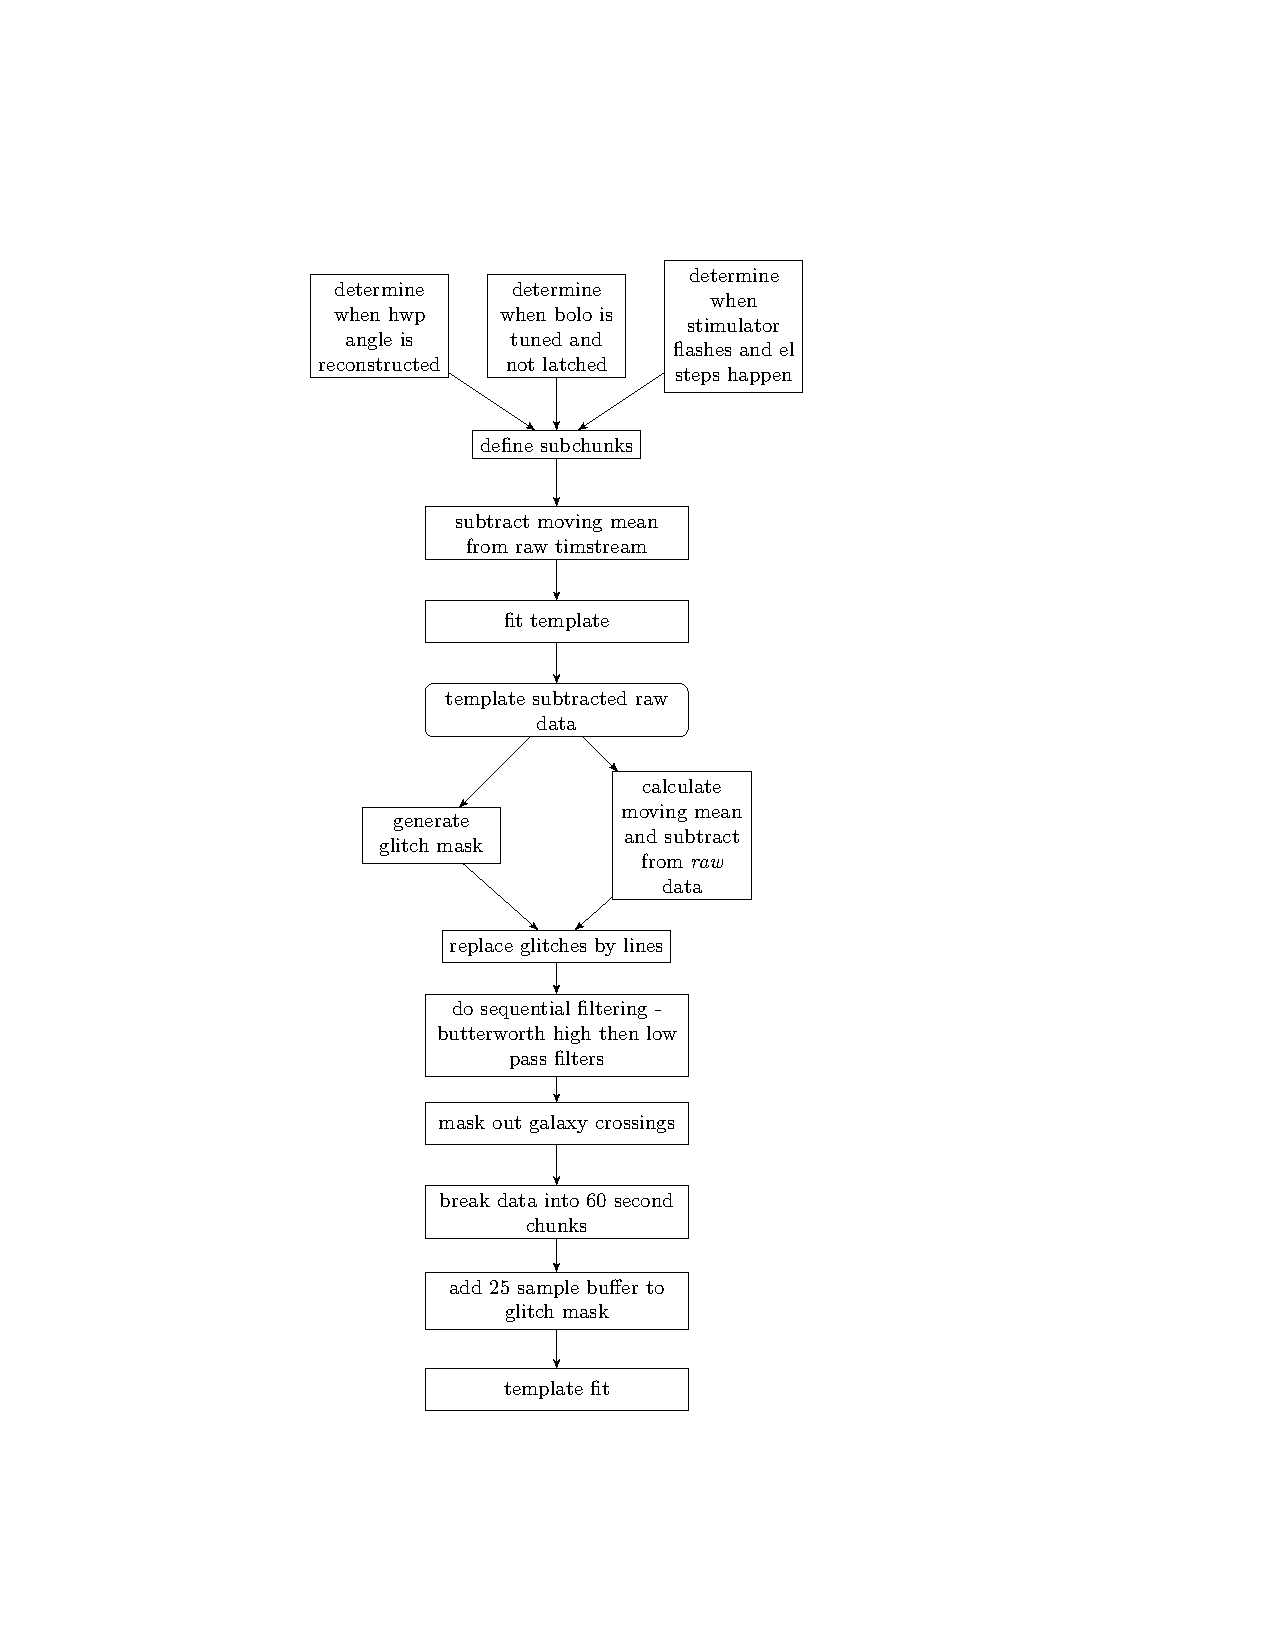
\includegraphics[width=0.6\columnwidth]{figures/mpi_new_block.pdf}
%\caption{Modified template fit flowchart, optimized for computing efficiency.}
%\label{fig:mpi_fit_flow}
%\end{center}
%\end{figure}


%%%%%%%%%%%%%%%%%%%%%%%%%%%%%%%%%%%%%%%%%%%%%%%%%%%%%%%%%%%%%%%%%%%%%%%%%%%%%%%%
